\documentclass[12pt, a4paper]{article}
\usepackage{amsmath}
\usepackage{amsfonts}
\usepackage{amsthm}
\usepackage{mathtools}
\newtheorem{theorem}{Theorem}[section]
\newtheorem{definition}{Definition}[section]
\numberwithin{equation}{section}
\usepackage{pgfplots}
\pgfplotsset{width=10cm,compat=1.9}
\graphicspath{ {img/} }
\DeclareGraphicsExtensions{.png}

\title{Recurrent Neural Networks}
\author{Kristian Wichmann}

\begin{document}
\maketitle

This follows Goodfellow and Bengio's book, borrowing/adapting a lot of the illustrations from this.

\section{Simple cyclical graph}

Image a situation, where a state $s=s^{(t)}$ depends on "time" $t$. Here $t$ is discrete, a whole number, usually, running from 1 to $\tau$. Further assume, that each time step is connected to the next through the same function:
\begin{equation}
s^{(t)}=f(s^{(t-1)},\theta)
\end{equation}
I.e., there is only an explicit dependence on the state from the last time step. Here $\theta$ is a shorthand for any parameters in the model. The unfolded graph of this model is shown in figure \ref{fig:cyclical_graph}.

\begin{figure}
\centering
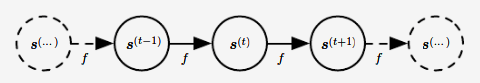
\includegraphics[width=\textwidth]{cyclical_graph}
\caption{Simple cyclical graph.}
\label{fig:cyclical_graph}
\end{figure}

\subsection{Cyclical graph with input}
To elaborate on this model, assume that at each time step, there is also some kind of input $x^{(t)}$. So now the state - now called $h^{(t)}$ for hidden state - depends on this as well:

\begin{equation}
s^{(t)}=f(s^{(t-1)}, x^{(t)},\theta)
\end{equation}

Figure \ref{fig:cyclical_with_input} shows both the folded and unfolded versions of this model.

\begin{figure}
\centering
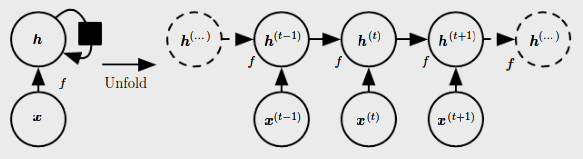
\includegraphics[width=\textwidth]{cyclical_with_input}
\caption{Cyclical graph with input.}
\label{fig:cyclical_with_input}
\end{figure}

\subsection{Cyclical graph with both input and output}
Finally, we would also like to model to provide some kind of output. We will assume there's output at every step, but in some applications, such as classification, we usually only care about the final output. 

\begin{figure}
\centering
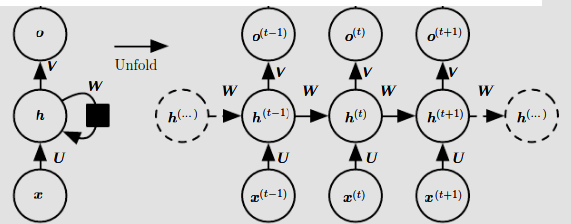
\includegraphics[width=\textwidth]{cyclical_input_output}
\caption{Cyclical graph with input as well as output.}
\label{fig:cyclical_input_output}
\end{figure}

Such a model is shown in figure \ref{fig:cyclical_input_output}. Here, the output at time $t$ depends only on the hidden state:
\begin{equation}
o^{(t)}=o(h^{(t)})
\end{equation}

\section{Recurrent neural networks}
As in feed forward neural networks, we will consider cases where the functions involved are linear followed by some kind of non-linearity. There's several ways to do this. We will explore some of them here.

\end{document}